\documentclass[tikz,border=5pt]{standalone}
\usepackage[T1]{fontenc}
\usepackage{lmodern,amsmath,amssymb}
\usetikzlibrary{arrows.meta,calc,positioning,fit,backgrounds,shapes.geometric,matrix,decorations.pathreplacing,patterns}
\definecolor{ink}{gray}{0.08}
\definecolor{wash}{gray}{0.965}
\definecolor{soft}{gray}{0.45}
\tikzset{box/.style={draw=ink,line width=.65pt,fill=white,align=center,inner sep=4pt,outer sep=0pt,font=\small},flow/.style={draw=ink,line width=.65pt,-{Latex[length=1.8mm,width=1.3mm]},rounded corners=2pt},annotation/.style={font=\scriptsize,text=soft,align=center},groupbox/.style={draw=soft,dashed,line width=.45pt,fill=wash}}
\begin{document}
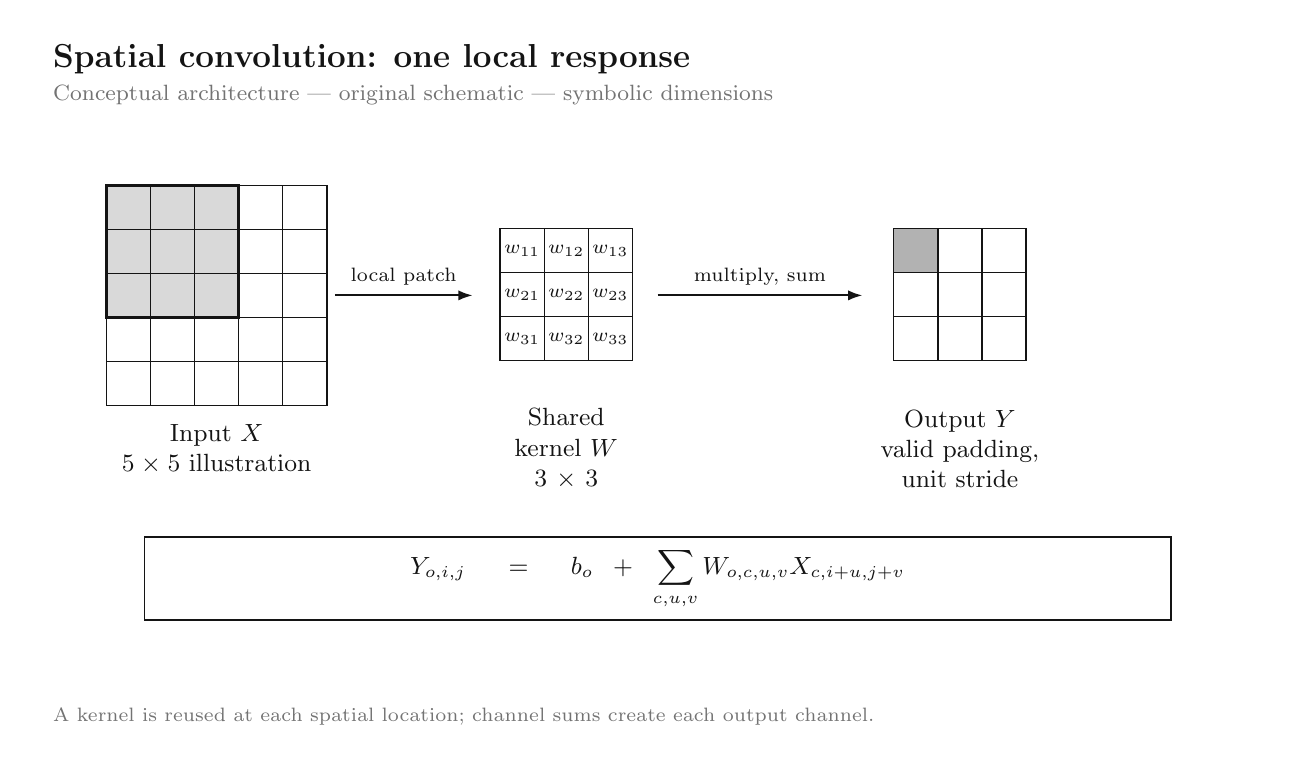
\begin{tikzpicture}[x=1cm,y=-1cm,font=\rmfamily,text=ink]

\path[use as bounding box] (0,0) rectangle (16,9);
\node[anchor=west,font=\large\bfseries] at (.2,.4) {Spatial convolution: one local response};
\node[anchor=west,font=\footnotesize,text=soft] at (.2,.85) {Conceptual architecture | original schematic | symbolic dimensions};
\begin{pgfonlayer}{background}
\end{pgfonlayer}
\node[align=center,inner sep=0pt,outer sep=0pt,font=\small,minimum width=3cm,minimum height=0.7cm,text width=2.75cm] (input) at (2.4,5.35) {Input $X$\par $5\times5$ illustration};
\node[align=center,inner sep=0pt,outer sep=0pt,font=\small,minimum width=2.6cm,minimum height=0.7cm,text width=2.35cm] (kernel) at (6.84,5.35) {Shared kernel $W$\par $3\times3$};
\node[align=center,inner sep=0pt,outer sep=0pt,font=\small,minimum width=3.5cm,minimum height=0.7cm,text width=3.25cm] (output) at (11.84,5.35) {Output $Y$\par valid padding, unit stride};
\node[box,minimum width=13cm,minimum height=1.0cm,text width=12.75cm] (equation) at (8,7.0) {$Y_{o,i,j}=b_o+\displaystyle\sum_{c,u,v} W_{o,c,u,v}X_{c,i+u,j+v}$};
\begin{pgfonlayer}{background}
\end{pgfonlayer}
\fill[black!15] (1.0,2.0) rectangle (1.56,2.56);
\fill[black!15] (1.56,2.0) rectangle (2.12,2.56);
\fill[black!15] (2.12,2.0) rectangle (2.68,2.56);
\fill[black!15] (1.0,2.56) rectangle (1.56,3.12);
\fill[black!15] (1.56,2.56) rectangle (2.12,3.12);
\fill[black!15] (2.12,2.56) rectangle (2.68,3.12);
\fill[black!15] (1.0,3.12) rectangle (1.56,3.68);
\fill[black!15] (1.56,3.12) rectangle (2.12,3.68);
\fill[black!15] (2.12,3.12) rectangle (2.68,3.68);
\draw[ink,line width=.45pt] (1.0,2.0) rectangle (3.8000000000000003,4.800000000000001);
\draw[ink,line width=.45pt] (1.56,2.0) -- (1.56,4.800000000000001);
\draw[ink,line width=.45pt] (2.12,2.0) -- (2.12,4.800000000000001);
\draw[ink,line width=.45pt] (2.68,2.0) -- (2.68,4.800000000000001);
\draw[ink,line width=.45pt] (3.24,2.0) -- (3.24,4.800000000000001);
\draw[ink,line width=.45pt] (1.0,2.56) -- (3.8000000000000003,2.56);
\draw[ink,line width=.45pt] (1.0,3.12) -- (3.8000000000000003,3.12);
\draw[ink,line width=.45pt] (1.0,3.68) -- (3.8000000000000003,3.68);
\draw[ink,line width=.45pt] (1.0,4.24) -- (3.8000000000000003,4.24);
\draw[ink,line width=1.1pt] (1,2) rectangle (2.68,3.68);
\draw[ink,line width=.45pt] (6.0,2.55) rectangle (7.68,4.23);
\draw[ink,line width=.45pt] (6.5600000000000005,2.55) -- (6.5600000000000005,4.23);
\draw[ink,line width=.45pt] (7.12,2.55) -- (7.12,4.23);
\draw[ink,line width=.45pt] (6.0,3.11) -- (7.68,3.11);
\draw[ink,line width=.45pt] (6.0,3.67) -- (7.68,3.67);
\node[font=\scriptsize] at (6.28,2.83) {$w_{11}$};
\node[font=\scriptsize] at (6.84,2.83) {$w_{12}$};
\node[font=\scriptsize] at (7.4,2.83) {$w_{13}$};
\node[font=\scriptsize] at (6.28,3.3899999999999997) {$w_{21}$};
\node[font=\scriptsize] at (6.84,3.3899999999999997) {$w_{22}$};
\node[font=\scriptsize] at (7.4,3.3899999999999997) {$w_{23}$};
\node[font=\scriptsize] at (6.28,3.95) {$w_{31}$};
\node[font=\scriptsize] at (6.84,3.95) {$w_{32}$};
\node[font=\scriptsize] at (7.4,3.95) {$w_{33}$};
\fill[black!30] (11.0,2.55) rectangle (11.56,3.11);
\draw[ink,line width=.45pt] (11.0,2.55) rectangle (12.68,4.23);
\draw[ink,line width=.45pt] (11.56,2.55) -- (11.56,4.23);
\draw[ink,line width=.45pt] (12.120000000000001,2.55) -- (12.120000000000001,4.23);
\draw[ink,line width=.45pt] (11.0,3.11) -- (12.68,3.11);
\draw[ink,line width=.45pt] (11.0,3.67) -- (12.68,3.67);
\draw[flow] (3.9,3.4) -- node[above,font=\scriptsize] {local patch} (5.65,3.4);
\draw[flow] (8.0,3.4) -- node[above,font=\scriptsize] {multiply, sum} (10.6,3.4);
\node[anchor=west,align=left,font=\scriptsize,text=soft,text width=15.6cm] at (.2,8.75) {A kernel is reused at each spatial location; channel sums create each output channel.};
\end{tikzpicture}
\end{document}
